\figcheckinputs{}
\expanded{\noexpand\begin{figure}[\figinputPos]}
    \centering
    \begin{subfigure}[t]{\figinputWidth}
        \centering
        \adjustbox{valign=t}{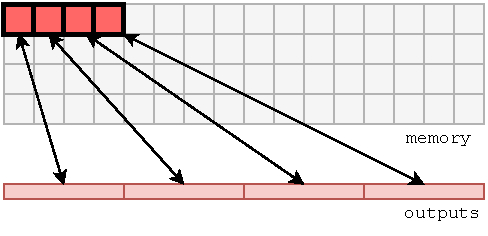
\includegraphics[width=\textwidth]{Figures/RVV_mem_unit_noseg.pdf}}
        \caption{Simple vector element to address mapping}
        \label{fig:RVV_mem_unit_noseg}
    \end{subfigure}
    \hfill
    \begin{subfigure}[t]{\figinputWidth}
        \centering
        \adjustbox{valign=t}{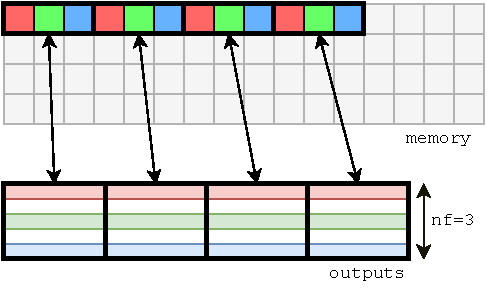
\includegraphics[width=\textwidth]{Figures/RVV_mem_unit_3seg.pdf}}
        \caption{Element-address mapping for segmented access}
        \label{fig:RVV_mem_unit_3seg}
    \end{subfigure}
    
    \begin{subfigure}[t]{\figinputWidth}
        \centering
     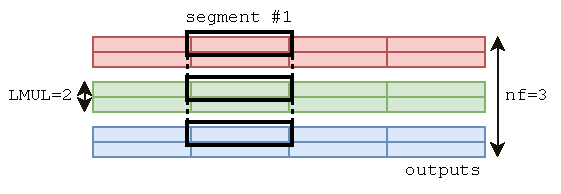
\includegraphics[width=\textwidth]{Figures/RVV_mem_lmul_3seg.pdf}
        \caption{Example of segment mapping for \code{LMUL > 1}}
        \label{fig:RVV_mem_lmul_3seg}
    \end{subfigure}
    \caption{Comparison between segmented and unsegmented accesses\\For readability, the vector registers are 2x as wide}
    \label{fig:RVV_mem_unit}
\end{figure}